\section{Problem Statement}
Towards the end of 2019, a novel virus emerged and spread throughout the city of Wuhan in China. A few months later, on 11th March 2020, the World Health Organization (WHO) officially declared that the SARS-CoV-2 virus has caused a global pandemic. Nearly two years later, the Covid-19 virus still poses a threat to humanity despite the countless efforts to thwart its spread and eliminate the virus through vaccinations. To this day, our general understanding of viruses is quite limited as people fail to understand how viruses infect humans and how they could potentially cause epidemics and pandemics by spreading through infected individuals. In our project, we aim to educate students about what viruses are, how they infect humans and how they can cause epidemics and pandemics.

\section{Proposed Solution}
In order to understand the mechanisms of the SARS-CoV-2 virus and how to prepare ourselves for future epidemics/pandemics, we plan on educating the population, especially students, about what a virus is, how it works, how it spreads, and its ability to mutate to ensure its survival through an AR platform. This will be done using an ecosystem of interactive models, games, and simulations in AR to ensure that the students don’t just learn for the sake of school but because their curiosity is peaked.

\section{Intended User}
Middle School and High School students who have access to a smartphone and internet.

\section{Project gantt chart and deliverables}
\subsection{Gantt Chart}
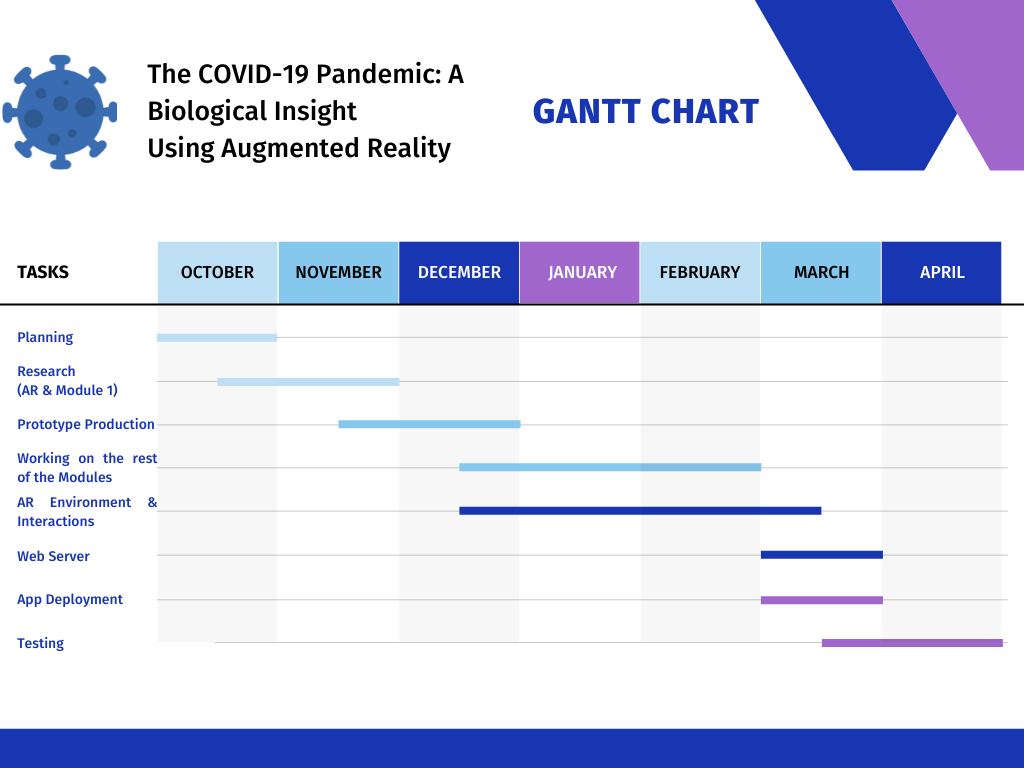
\includegraphics[scale=0.5]{ganttChart.png}

\subsection{Deliverables}
\begin{enumerate}
    \item Physical booklet to access the content 
    \item Mobile application with all the AR games and simulations
\end{enumerate}


\section{Key Challenges}
The main challenge for the team is to learn AR as it is something that we’re new to. However, given the multiple resources available online, the team will be able to learn a sufficient amount on the subject for this project. Apart from this, our project will encounter certain hardware limitations. We currently do not possess any Apple devices. Therefore the team has decided to first develop the app for Android and move on to iOS if time permits.